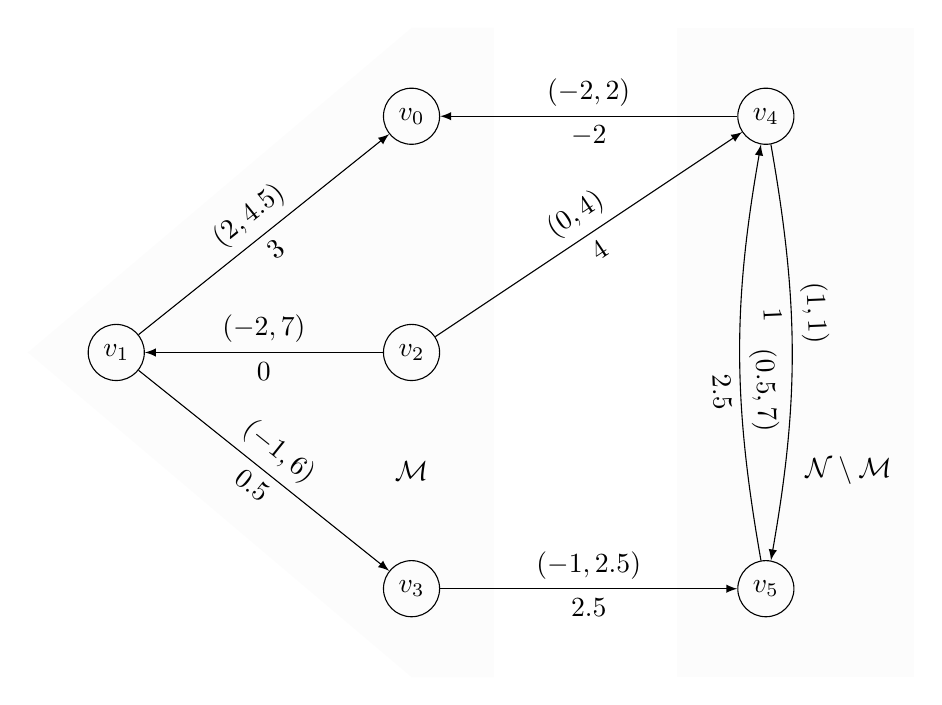
\begin{tikzpicture}[scale = 1.5]
  \fill[
    opacity=0.2,
    lightgray!20
  ] (-1.75, 0) -- (1.5, 2.75) -- (2.2, 2.75) -- (2.2, -2.75) -- (1.5, -2.75) -- cycle  ;
  \fill[
    opacity=0.2,
    lightgray!20
  ] (3.75, 2.75) -- (5.75, 2.75) -- (5.75, -2.75) -- (3.75, -2.75) -- cycle  ;
  
  \draw node[circle, draw] (v0) at (1.5, 2) {$v_0$};
  \draw node[circle, draw] (v2) at (1.5, 0) {$v_2$};
  \draw node[circle, draw] (v3) at (1.5, -2) {$v_3$};
  \draw node[circle, draw] (v1) at (-1, 0) {$v_1$};
  \draw node[circle, draw] (v4) at (4.5, 2) {$v_4$};
  \draw node[circle, draw] (v5) at (4.5, -2) {$v_5$};

  \draw[-latex] (v1) -- (v0) node[
    midway,
    sloped,
    above
  ] {$(2, 4.5)$} node[midway, sloped, below] {$3$};
  \draw[-latex] (v2) -- (v1)
    node[midway, above] {$(-2, 7)$}
    node[midway, below] {$0$};
    
  \draw[-latex] (v3) -- (v5)
    node[midway, above] {$(-1, 2.5)$}
    node[midway, below] {$2.5$};

  \draw[-latex] (v2) -- (v4)
    node[midway, sloped, above] {$(0, 4)$}
    node[midway, sloped, below] {$4$};
    
  \draw[-latex] (v4) to[bend left=10]
    node[midway, sloped, above, pos=0.4] {$(1, 1)$}
    node[midway, sloped, below, pos=0.4] {$1$}(v5) ;
    
  \draw[-latex] (v5) to[bend left=10]
    node[midway, sloped, above, pos=0.4] {$(0.5, 7)$}
    node[midway, sloped, below, pos=0.4] {$2.5$}(v4);
    
  \draw[-latex] (v1) -- (v3)
    node [midway, sloped, above] {$(-1, 6)$}
    node [midway, sloped, below] {$0.5$};
    
  \draw[-latex] (v4) -- (v0)
    node[midway, above] {$(-2, 2)$}
    node[midway, below] {$-2$};

  \node at (1.5, -1) {$\mathcal{M}$};
  \node at (5.2, -1) {$\mathcal{N} \setminus \mathcal{M} $};

\end{tikzpicture}

